\documentclass[11pt]{article}

	\usepackage{amsmath}
	\usepackage{mathtools}
	
    \title{\textbf{Práctica 2}}
    \author{Adrián Racero Serrano}
    \date{\today}
    
    \addtolength{\topmargin}{-3cm}
    \addtolength{\textheight}{3cm}
\usepackage{graphicx}
\begin{document}

\maketitle
\thispagestyle{empty}

\section*{Ejercicio 1}
Consider the language over the alphabet \{a, b\} that only contains the string a.
\begin{description}
\addtolength{\itemindent}{0.80cm}
\itemsep0em 
\item[a.] Build a DFA that recognizes this language and rejects all those strings that do not belong to the language.
\item[b.] Test the automaton that you have created by introducing 6 chains.
\end{description}
\begin{flushleft}\end{flushleft}
a)
\begin{equation*}
M = (\{q_{0},q_{1},q_{2}\}, 
\{a,b\}, \delta, q_0, \{q_1\})
\end{equation*}

\begin{table}[h!]
\begin{tabular}{c|c|c}
  $\delta(q,\sigma)$ & $a$ & $b$\\
  \hline
  $q_0$& $q_1$ & $q_2$\\
  \hline
  $q_1$& $q_2$ & $q_2$\\
  \hline
  $q_2$& $q_2$ & $q_2$
\end{tabular}
\end{table}

\begin{figure}[htp]
\centering
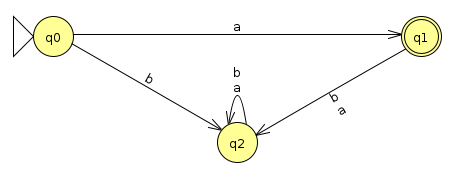
\includegraphics[scale=0.60]{only-a.png}
\label{}
\end{figure}

\newpage

\begin{flushleft}\end{flushleft}
b)
\begin{figure}[htp]
\centering
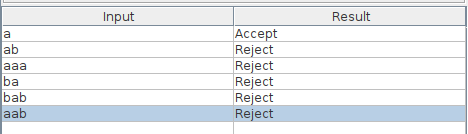
\includegraphics[scale=0.60]{test-only-a.png}
\label{}
\end{figure}

\newpage
\begin{flushleft}\end{flushleft}
\section*{Ejercicio 2}
Finite automaton in Octave:
\begin{description}
\addtolength{\itemindent}{0.80cm}
\itemsep0em 
\item[a)] Open the Octave finiteautomata.m script and test it with the given example (see script help) in the GitHub repository.
\item[b)] Specify in finiteautomata.json the automaton created in Activity 1 and test it with the script!
\end{description}

\begin{flushleft}\end{flushleft}
a)

\begin{figure}[htp]
\centering
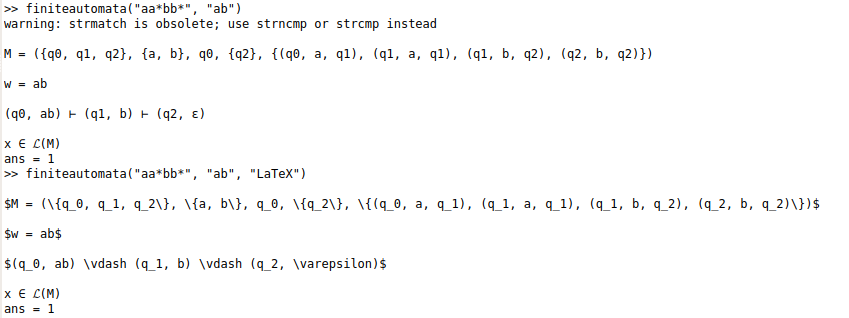
\includegraphics[scale=0.50]{ejemplo-octave.png}
\label{}
\end{figure}

\newpage
\begin{flushleft}\end{flushleft}
b)
\\\\
$M = (\{q_0, q_1, q_2\}, \{a, b\}, q_0, \{q_1\}, \{(q_0, a, q_1), (q_0, b, q_2), (q_1, a, q_2), (q_1, b, q_2), (q_2, a, q_2), (q_2, b, q_2)\})$

$w = a$

$(q_0, a) \vdash (q_1, \varepsilon)$
\begin{figure}[htp]
\centering
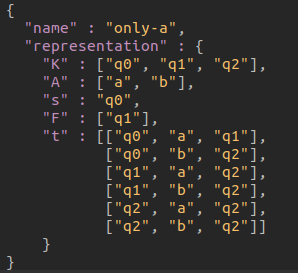
\includegraphics[scale=0.60]{only-a-octave.png}
\label{}
\end{figure}

\begin{figure}[htp]
\centering
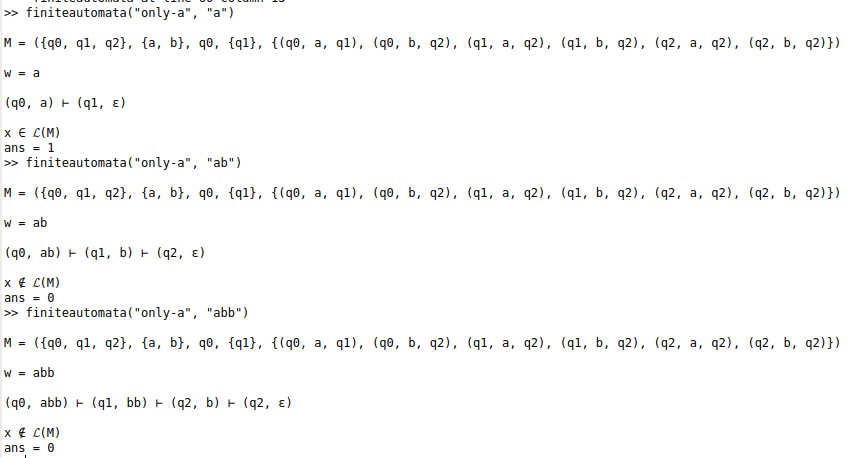
\includegraphics[scale=0.5]{test-only-a-octave.png}
\label{}
\end{figure}

\end{document}

